% !TeX root = ../main.tex
\section{Room-level conditional shear wall layout generation framework}
\label{sec:methodology}

\begin{figure*}[t]
\centering
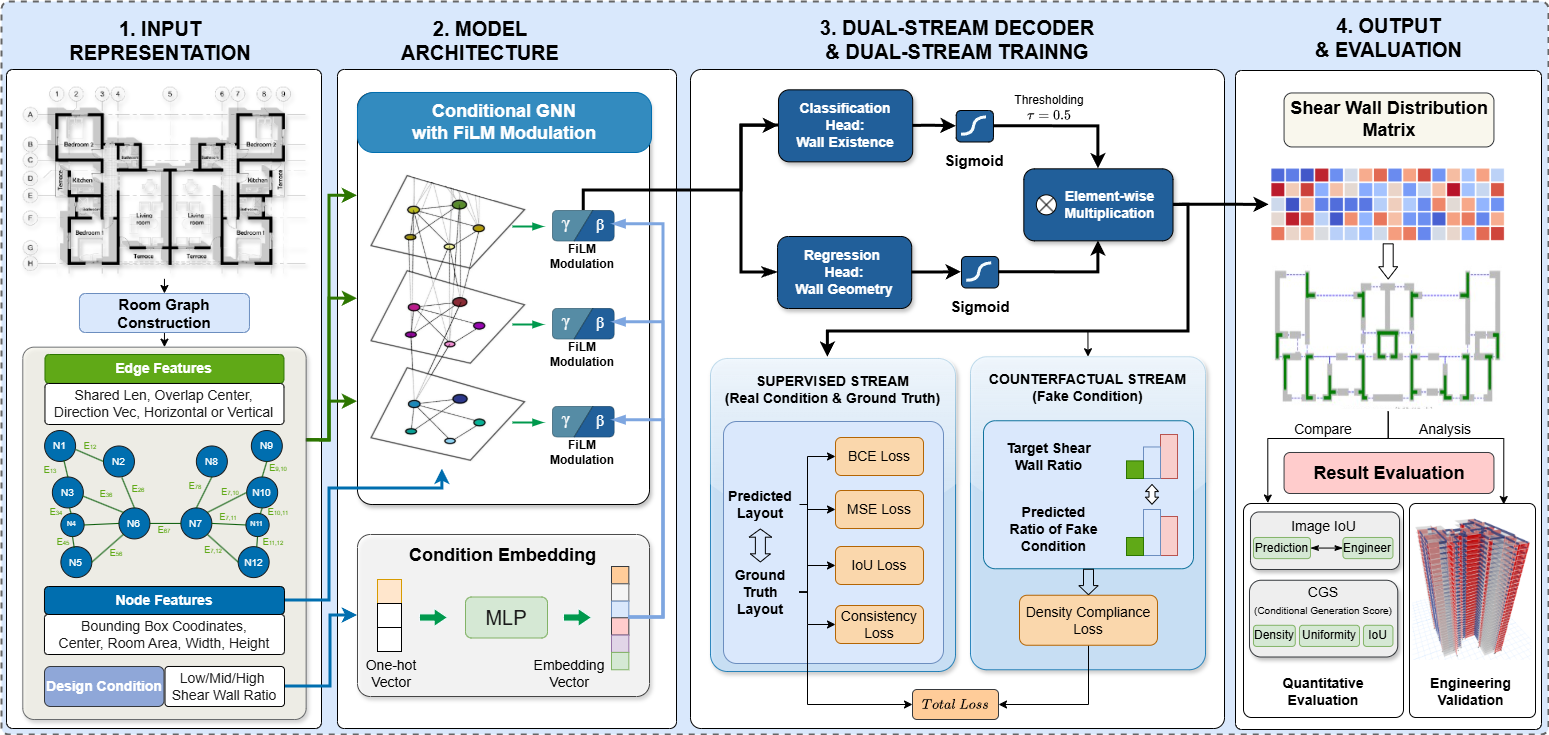
\includegraphics[width=\textwidth]{framework.pdf}
\caption{The overall framework of the proposed room-level conditional shear wall layout generation method. \textcolor{red}{The supervised stream learns from matched floor-plan--layout pairs, while the cross-condition stream uses mismatched condition inputs with density regularization to improve condition responsiveness under limited paired data.}}
\label{fig:framework}
\end{figure*}


To address the challenges of semantic alignment and conditional controllability in shear wall design, this study proposes a unified generative framework, RC-GNN (Room-level Conditional Graph Neural Network), as illustrated in Fig.~\ref{fig:framework}. The pipeline is organized into four stages:

(1) Input representation: Raw computer-aided design (CAD) plans are converted into room-adjacency graphs, which explicitly encode architectural spaces and design conditions as node and edge features.

(2) Conditional shear wall layout prediction: The graph is processed by a GATv2 backbone for spatial feature extraction, with FiLM used for condition injection \cite{perezFiLMVisualReasoning2018}.

(3) Dual-stream decoding and training: A decoupled prediction head outputs wall existence and geometry, and the model is optimized by combining supervised learning on matched pairs with cross-condition regularization on unmatched conditions.

(4) Output and evaluation: Predicted probability matrices are post-processed into vectorized structural layouts for quantitative evaluation and engineering validation.


For readability, key symbols used throughout this section are summarized in Table~\ref{tab:notation}.


\begin{table}[t]
\centering
\caption{Notation summary}
\label{tab:notation}
\small
\begin{tabularx}{\columnwidth}{lX}
\toprule
Symbol & Definition \\
\midrule
$\mathcal{P}$ & Architectural floor plan \\
$G = (\mathcal{V}, \mathcal{E})$ & Room adjacency graph \\
$\mathcal{V} = \{v_1, \ldots, v_N\}$ & Set of $N$ room nodes \\
$\mathcal{E} \subseteq \mathcal{V} \times \mathcal{V}$ & Set of adjacency edges \\
$\mathbf{X} \in \mathbb{R}^{N \times D_v}$ & Node feature matrix ($D_v = 25$) \\
$\mathbf{A} \in \mathbb{R}^{|\mathcal{E}| \times D_e}$ & Edge attribute matrix ($D_e = 8$) \\
$c \in \{0, 1, 2\}$ & Design condition index (low/medium/high) \\
$\mathbf{z}_c \in \mathbb{R}^{D_c}$ & Condition embedding vector ($D_c = 32$) \\
$\mathbf{Y} \in [0,1]^{N \times 16}$ & Ground-truth shear wall layout matrix \\
$\hat{\mathbf{Y}} \in [0,1]^{N \times 16}$ & Predicted shear wall layout matrix \\
$\mathbf{M} \in \{0,1\}^{N \times 16}$ & Constraint mask (1 = wall placement permitted) \\
$\mathcal{N}_i$ & Neighborhood of node $v_i$ \\
\bottomrule
\end{tabularx}
\end{table}

\subsection{Room-based graph representation}
\label{subsec:room_graph}

The choice of graph representation is critical for capturing the architectural logic governing shear wall placement. Traditional approaches typically employ a component-level representation, where geometric components (e.g., wall segments) serve as edges and their intersections as nodes \cite{zhaoIntelligentDesignShear2023b,zhaoDesignconditioninformedShearWall2023d}. While this preserves detailed topology, it suffers from semantic gaps and computational redundancy.

\begin{figure*}[t]
\centering

\includegraphics[width=0.8\textwidth]{graph_comparison.png}
\caption{Comparison of graph representations for the same residential floor plan.}
\label{fig:graph_comparison}
\end{figure*}

As illustrated in Fig.~\ref{fig:graph_comparison}, the component-level approach leads to an excessive graph scale. A standard residential plan can produce a graph with more than 100 nodes and edges (Fig.~\ref{fig:graph_comparison}a), yet individual wall segments carry little information about the functional spaces they enclose. In contrast, the proposed room-level formulation (Fig.~\ref{fig:graph_comparison}b) models functional rooms as nodes and their physical adjacencies as edges.

Modeling floor plans at the room level therefore allows the learning problem to incorporate architectural semantics and boundary feasibility in a compact representation, while remaining compatible with standard message-passing GNNs.
It should be noted that the current formulation assumes rectangular room geometry; non-rectangular spaces are pre-processed via rectilinear decomposition before graph construction (Section~\ref{subsubsec:graph_construction}), and the resulting virtual partition boundaries are excluded from wall placement through the constraint mask. This choice is consistent with prior zoning used to simplify structural design spaces \cite{Claessens_2020,Liu_2021}.
\textcolor{red}{The proposed room-level formulation is therefore designed primarily for regular high-rise residential, apartment, hotel, and dormitory-type buildings, where rooms are mostly orthogonal and can be represented by rectangular or rectilinearly decomposed regions. In such cases, shear wall candidates are usually constrained by room boundaries, and room-level nodes provide a compact representation that is aligned with engineering practice. However, this abstraction may lose fine-grained local geometric details compared with component-level graphs. For floor plans with highly irregular spaces, long and narrow corridors, fragmented public areas, or many small local wall segments, rectilinear decomposition may introduce virtual partitions that do not correspond to actual structural decisions. Although these virtual boundaries can be excluded by the constraint mask, they may still affect feature aggregation and model learning.}


\subsubsection{Graph construction from floor plans}
\label{subsubsec:graph_construction}

Given an architectural floor plan $\mathcal{P}$ in CAD format, the room adjacency graph $G = (\mathcal{V}, \mathcal{E}, \mathbf{X}, \mathbf{A})$ is constructed through the following procedure. \textcolor{red}{The preprocessing stage converts CAD primitives into room polygons, opening-aware boundary constraints, and graph connectivity.}

\textbf{Step 1: Space Partitioning.} \textcolor{red}{Wall, door, window, and beam entities are first parsed from the CAD drawing according to their layer types. Double-line wall boundaries are converted into wall centerlines, and door/window embedded segments are projected onto their host walls as openings. The wall centerlines are then calibrated by closing small drafting gaps, merging nearly collinear segments, and adjusting intersections within a geometric tolerance, producing a connected floor-plan skeleton. Polygonizing this calibrated skeleton yields closed spatial regions.} To process complex architectural layouts, a rectilinear decomposition algorithm is applied to partition any non-rectangular regions (e.g., L-shaped or T-shaped spaces) into a set of axis-aligned rectangular sub-regions. \textcolor{red}{Corridors and circulation spaces follow the same rule: rectangular regions are kept as single nodes, whereas irregular connected regions are decomposed into rectangular sub-regions so that the fixed 16-dimensional boundary representation remains applicable.}

\textbf{Step 2: Room Node Registration.} Each resulting rectangular sub-region with an area exceeding a minimum threshold is registered as a room node $v_i$. \textcolor{red}{Openings are associated with the corresponding room-boundary segments according to geometric overlap, so that wall placement is prohibited where doors or windows interrupt a boundary. During dataset preparation, room partitions were manually checked; visually enclosed regions that were already covered by surrounding room partitions and did not introduce an independent room or additional physical boundary were not registered as separate nodes.} Partition boundaries introduced during the decomposition step are treated as virtual edges that carry no structural meaning; consequently, their corresponding entries in the constraint mask $\mathbf{M}$ are set to zero to strictly prohibit shear wall placement along these artificial lines. \textcolor{red}{Fig.~\ref{fig:output_param}c illustrates this masking rule: feasible physical boundary slots are retained, whereas openings and virtual decomposition boundaries are marked as non-buildable.}

\textbf{Step 3: Adjacency Edge Construction.} For each pair of rooms, the shared physical boundary length $l_{ij}$ is computed. An adjacency edge $e_{ij}$ is added to $\mathcal{E}$ only if $l_{ij}$ exceeds a physical threshold $\tau_{adj}$ (set to 400 mm), which filters out minor or accidental structural contacts.

\textbf{Step 4: Attribute \& Label Mapping.} Finally, node features $\mathbf{X}$ and edge attributes $\mathbf{A}$ are computed based on the geometry and spatial relationships (detailed in Sections~\ref{subsubsec:node_features} and~\ref{subsubsec:edge_features}). \textcolor{red}{The feasible wall-boundary mask $\mathbf{M}$ is built by marking physical room boundaries as buildable and excluding openings and virtual decomposition boundaries.} For the training data, ground-truth shear wall locations are extracted from structural engineering drawings and precisely mapped to the 16-dimensional output representation (Section~\ref{subsubsec:output_param}). \textcolor{red}{During this mapping, the effective length of a shear wall is defined as the projected overlap length between an extracted structural wall segment and a feasible room-boundary slot. Overlaps on openings, non-buildable slots, or virtual decomposition boundaries are discarded by the mask, and multiple wall intervals on the same slot are merged before the final coverage ratio is computed.}

\subsubsection{Node feature design}
\label{subsubsec:node_features}

Each room node $v_i$ is associated with a 25-dimensional feature vector $\mathbf{x}_i \in \mathbb{R}^{25}$, which is formed by concatenating 9 geometric descriptors and 16 constraint indicators.
The normalized geometric feature vector is 9-dimensional, $\mathbf{x}_i^{geo}\in\mathbb{R}^{9}$, defined as
$(x_{min}, y_{min}, x_{max}, y_{max}, w, h, a, x_c, y_c)$, where $(x_{min},y_{min},x_{max},y_{max})$ are the bounding box coordinates, $w$ and $h$ are the bounding box width and height, $a$ is the room area, and $(x_c,y_c)$ is the room centroid.
All entries are normalized to $[0,1]$ within a floor plan.
Constraint information is represented by a 16-dimensional buildable mask $\mathbf{m}_i \in \{0,1\}^{16}$ that indicates whether each boundary segment permits shear wall placement.
\textcolor{red}{The mask follows the same ordering as the 16-dimensional output vector $\mathbf{y}_i$: the four room boundaries are ordered as top, right, bottom, and left; each boundary is divided into two half-segments; and each half-segment is represented by two directional coverage entries. Thus, every mask component $m_{ij}$ corresponds one-to-one to the output component $y_{ij}$, as visualized in Fig.~\ref{fig:output_param}c.}
Specifically, segments occupied by doors, windows, or other openings are marked as non-buildable (value 0), while remaining segments are marked as buildable (value 1).
Table~\ref{tab:node_features} summarizes the full feature specification.

\begin{table}[t]
\centering
\caption{Node feature specification}
\label{tab:node_features}
\small
\begin{tabularx}{\columnwidth}{llX}
\toprule
Category & Dim. & Features \\\midrule
Geometric & 4 & Bounding box $(x_{min}, y_{min}, x_{max}, y_{max})$, normalized \\
Geometric & 2 & Bounding-box size $(w, h)$, normalized \\
Geometric & 1 & Area $a$, normalized \\
Geometric & 2 & Centroid coordinates $(x_c, y_c)$, normalized \\
Constraint & 16 & Buildable mask $\mathbf{m}_i \in \{0,1\}^{16}$ \\
\bottomrule
\end{tabularx}
\end{table}

The constraint mask $\mathbf{m}_i$ is aligned with the output parameterization introduced in Section~\ref{subsubsec:output_param}, enabling the model to learn wall placement while explicitly respecting architectural openings. \textcolor{red}{Mask entries are also set to zero for virtual boundaries introduced by rectilinear decomposition, so these artificial boundaries are excluded from both training losses and final wall placement.}
All geometric features are normalized using min-max scaling computed over the training set to ensure consistent feature magnitudes.

Room function labels (e.g., bedroom, living room, kitchen) would in principle provide additional semantic cues for shear wall placement, as structural engineers routinely consider functional zoning when allocating lateral-load-resisting elements. However, the open-source dataset employed in this study does not include room-type annotations for individual spaces. In the current dataset, geometric cues and buildable-boundary constraints still provide substantial information because feasible wall locations are already strongly restricted by room shape, adjacency, and openings. The model can therefore learn meaningful placement patterns without explicit function labels, but it cannot distinguish cases in which rooms with similar geometry should be treated differently because of their usage. Functional labels are thus omitted in the present formulation due to data availability rather than because they are unimportant, and incorporating them remains a direct extension once annotated datasets become available.

\subsubsection{Edge feature design}
\label{subsubsec:edge_features}

Each edge $e_{ij}$ connecting adjacent rooms $v_i$ and $v_j$ is associated with an attribute vector $\mathbf{a}_{ij} \in \mathbb{R}^{8}$.
The edge feature vector is 8-dimensional and consists of the normalized shared boundary length, the normalized overlap centroid $(x_{ov},y_{ov})$ of the shared boundary, a 4-dimensional relative direction indicator (top/bottom/left/right), and a binary orientation flag indicating whether the shared boundary is horizontal.
The complete list of edge attributes is given in Table~\ref{tab:edge_features}.

\begin{table}[t]
\centering
\caption{Edge feature specification}
\label{tab:edge_features}
\small
\begin{tabularx}{\columnwidth}{llX}
\toprule
Feature & Dimension & Description \\\midrule
Shared length & 1 & Normalized length of the shared boundary between rooms $i$ and $j$ \\
Overlap centroid & 2 & Normalized centroid coordinates $(x_{ov}, y_{ov})$ of the shared boundary segment \\
Relative direction & 4 & One-hot encoding indicating the relative position (top/bottom/left/right) of the adjacent room \\
Orientation flag & 1 & Binary indicator of boundary orientation (1 = horizontal, 0 = vertical) \\
\bottomrule
\end{tabularx}
\end{table}

The directional encoding enables the model to learn orientation-specific patterns (e.g., walls more common on certain sides of rooms).

\subsubsection{Output parameterization}
\label{subsubsec:output_param}

The shear wall layout for each room $v_i$ is parameterized as a continuous vector $\mathbf{y}_i \in [0,1]^{16}$.
This parameterization captures wall placement along all four room boundaries with segment-level precision.
An 8-dimensional alternative would regress two coverage ratios for each of the four boundaries (e.g., measured from the two endpoints of each boundary).
However, this representation fails when a wall segment lies in the interior of a boundary without touching either endpoint, as both endpoint-based ratios would be close to zero and the wall could be incorrectly treated as absent.
To avoid this ambiguity, each boundary (top, right, bottom, left) is split at its midpoint into two half-segments, yielding 8 half-segments in total.
Each half-segment is then described by two ratios, which together provide sufficient flexibility to represent walls attached to an endpoint as well as walls located away from endpoints (Fig.~\ref{fig:output_param}).
For each half-segment $k \in \{1, \ldots, 8\}$, two values encode the wall coverage:

$r_k^{start}$ denotes the fraction of the half-segment covered by wall starting from the segment's origin.

$r_k^{end}$ denotes the fraction covered starting from the segment's terminus.

The complete output vector is:
\begin{align}
\mathbf{y}_i = [r_1^{start}, r_1^{end}, r_2^{start}, r_2^{end}, \ldots, r_8^{start}, r_8^{end}]
\end{align}
In practice, splitting each boundary into two halves already covers typical engineering layouts, since shear walls are rarely fragmented into many disjoint sub-segments along a single short boundary.
Further subdivision would increase output dimensionality while providing limited additional benefit, and is therefore not adopted in this work.

The resulting 16-dimensional vector $\mathbf{y}_i$ provides a continuous representation capable of encoding various wall configurations. Specifically, values of 1.0 denote full wall coverage, whereas intermediate values represent partial walls. \textcolor{red}{For each boundary slot, the ground-truth coverage ratio is obtained by dividing the effective shear wall length within that slot by the slot length; therefore, a value of 1.0 indicates full coverage and an intermediate value indicates partial coverage. These ratios form the ground-truth vector and are also used in density-related losses and scores.} This parameterization flexibly handles cases ranging from complete structural walls to boundaries containing openings, or simply non-structural partitions (represented by zero values), within a unified vector space.

Because adjacent rooms $v_i$ and $v_j$ each independently predict coverage on their shared boundary, their predictions may be mutually inconsistent.
During inference, this is resolved by taking the element-wise maximum of the two predictions for the corresponding boundary entries:
\begin{equation}
\hat{y}_{shared} = \max\!\left(\hat{\mathbf{y}}_i^{(side_j)},\; \hat{\mathbf{y}}_j^{(side_i)}\right),
\label{eq:boundary_union}
\end{equation}
where $side_j$ denotes the boundary slots of room $v_i$ that face room $v_j$, and vice versa.
This union rule avoids artificial wall fragmentation. If either room predicts a wall on the shared segment, the wall is retained in the final layout.
The topological consistency loss $\mathcal{L}_{cons}$ (Section~\ref{subsec:training_strategy}) encourages both rooms to reach compatible predictions during training, reducing the frequency and magnitude of such conflicts at inference time.

\begin{figure*}[t]
\centering
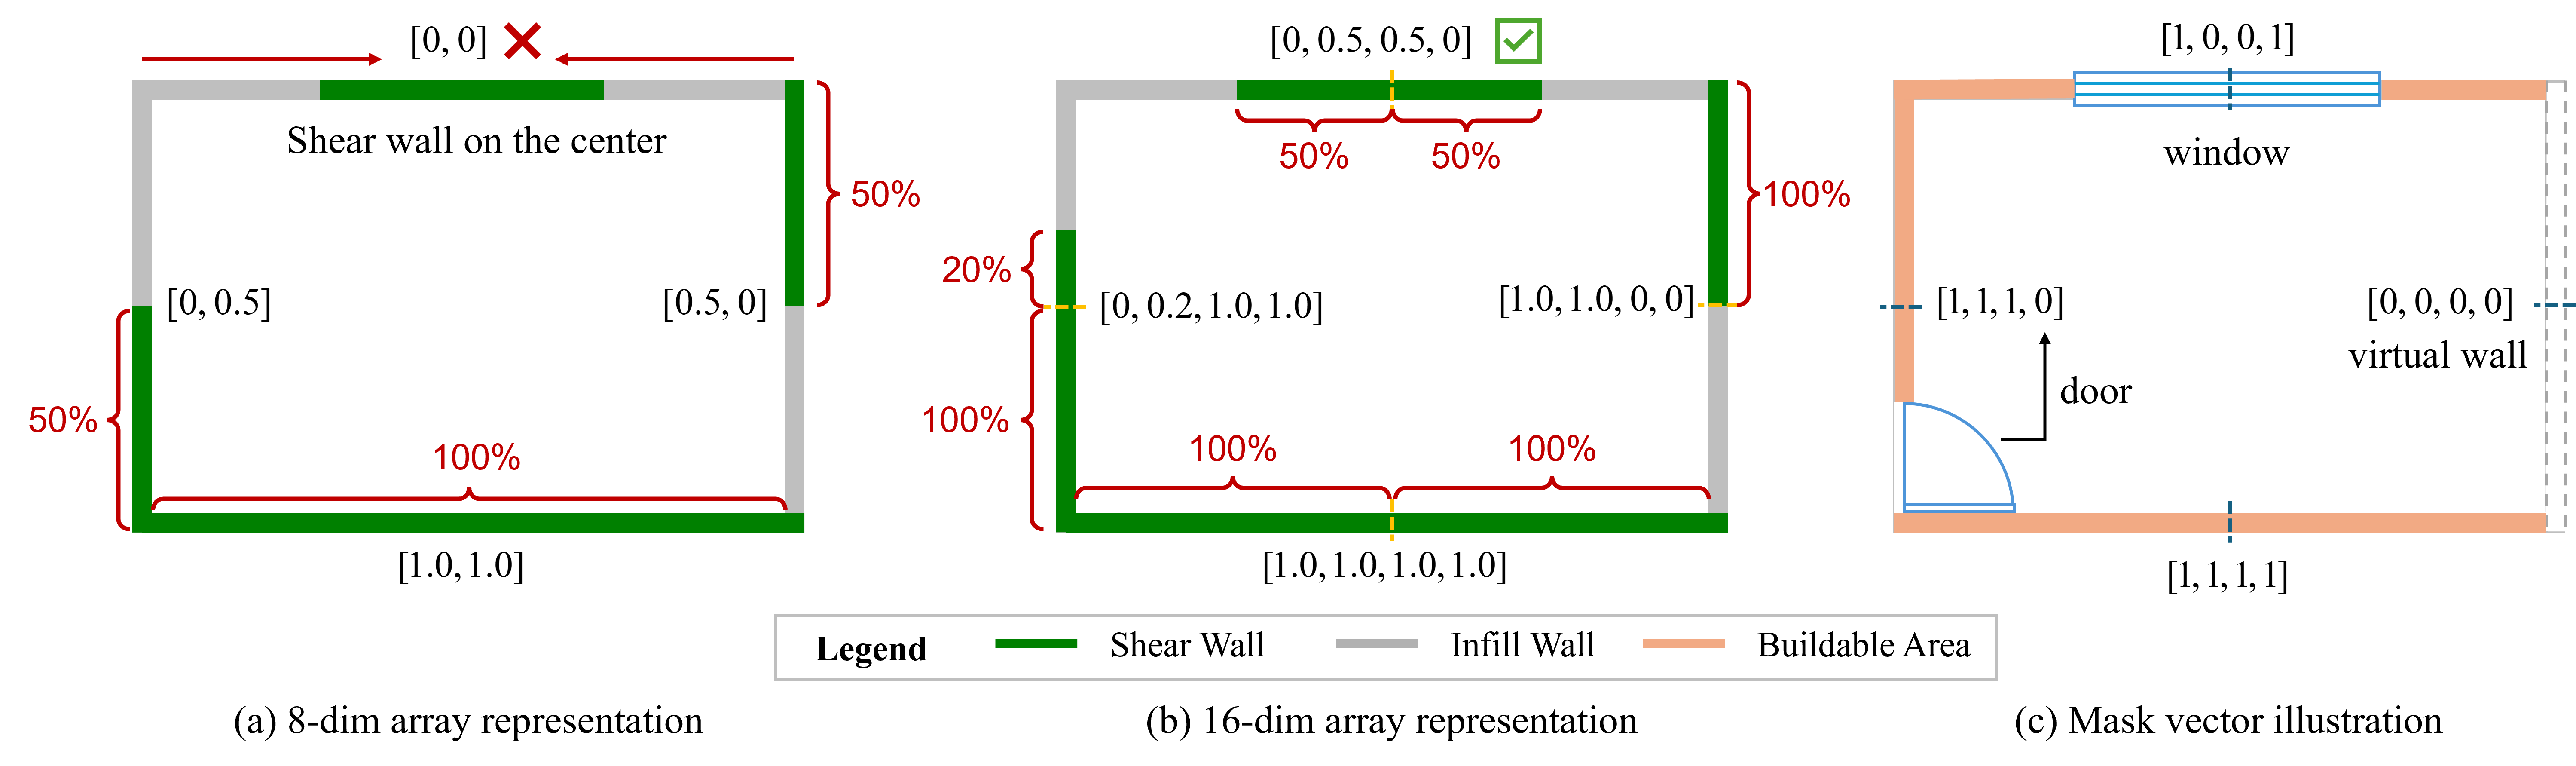
\includegraphics[width=0.85\textwidth]{output_param_and_mask.png}
\caption{Illustration of the 16-dimensional room-level output parameterization and the corresponding constraint mask.}
\label{fig:output_param}
\end{figure*}

\subsection{Problem Formulation}
\label{subsec:problem_formulation}

The shear wall layout generation task is formulated as conditional graph-to-matrix regression.
Given:
\begin{enumerate}[(\arabic*)]
\item Room adjacency graph $G = (\mathcal{V}, \mathcal{E}, \mathbf{X}, \mathbf{A})$ constructed from floor plan $\mathcal{P}$
\item Design condition $c \in \{0, 1, 2\}$ specifying target shear wall density category (low, medium, high)
\item Constraint mask $\mathbf{M} \in \{0,1\}^{N \times 16}$ indicating buildable locations
\end{enumerate}


The objective is to learn a parameterized mapping $f_\theta$:
\begin{equation}
\hat{\mathbf{Y}} = f_\theta(G, c)
\label{eq:method_mapping}
\end{equation}
that predicts the shear wall layout matrix $\hat{\mathbf{Y}} \in [0,1]^{N \times 16}$ approximating the ground-truth layout $\mathbf{Y}$ while respecting physical constraints encoded in $\mathbf{M}$.

The learning objective minimizes a composite loss:
\begin{equation}
\min_\theta \mathbb{E}_{(G, c, \mathbf{Y}) \sim \mathcal{D}} \left[ \mathcal{L}_{sup}(\hat{\mathbf{Y}}, \mathbf{Y}) + \lambda_{cond} \mathcal{L}_{cond}(\hat{\mathbf{Y}}, \mathbf{M}, c) \right]
\label{eq:method_objective}
\end{equation}
where $\mathcal{L}_{sup}$ denotes supervised reconstruction loss and $\mathcal{L}_{cond}$ denotes condition-aware regularization under architectural constraints. Detailed loss formulations are presented in Section~\ref{subsec:training_strategy}.

\subsection{Conditional graph neural network architecture}
\label{subsec:architecture}

The proposed architecture comprises three components: a GATv2-based encoder for spatial feature aggregation, a FiLM module for conditional injection, and a dual-head decoder for task-decoupled prediction.
Fig.~\ref{fig:network} illustrates the overall architecture.

\begin{figure*}[t]
\centering
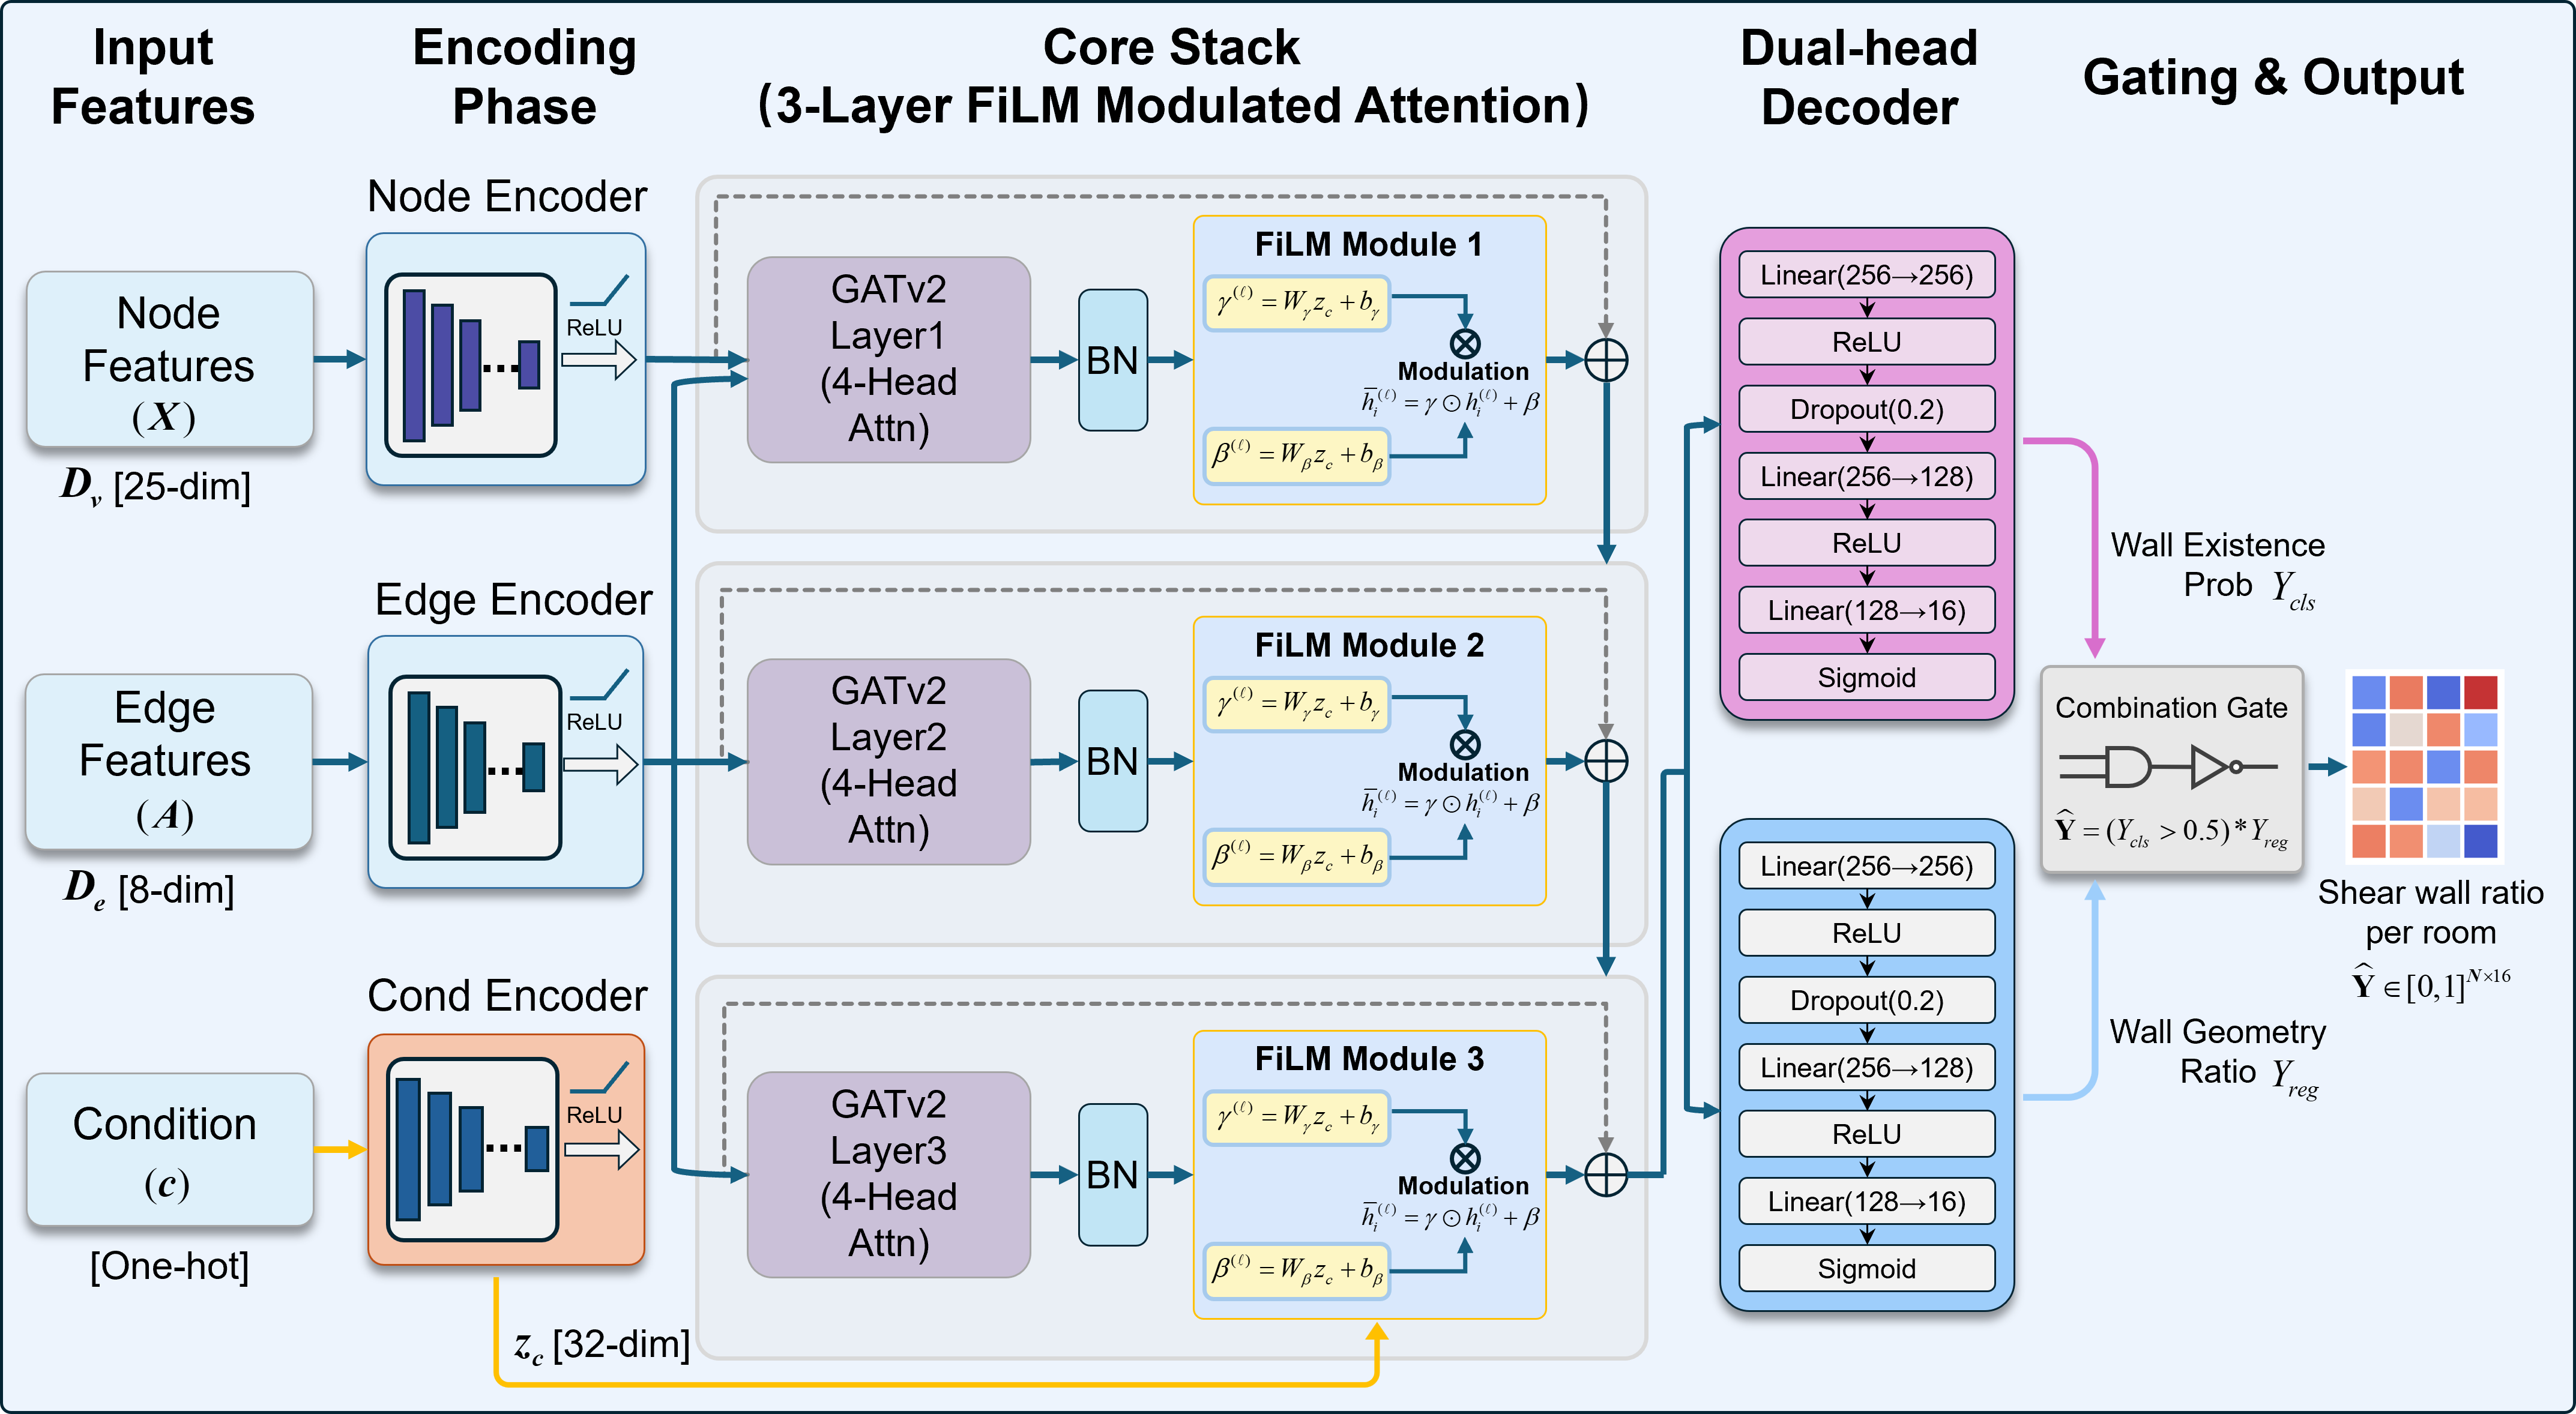
\includegraphics[width=\textwidth]{architecture.png} 
\caption{Model architecture diagram. The architecture consists of: (1) Node and edge encoders, (2) Three GATv2 layers with residual connections, (3) FiLM conditioning applied after each layer, (4) Dual-head decoder producing classification and regression outputs.}
\label{fig:network}
\end{figure*}

\subsubsection{Feature encoding}

Raw node and edge features are projected to a common hidden dimension $D_h = 256$:
\begin{align}
\mathbf{h}_i^{(0)} &= \text{ReLU}(\mathbf{W}_{node} \mathbf{x}_i + \mathbf{b}_{node}) \\
\mathbf{e}_{ij} &= \text{ReLU}(\mathbf{W}_{edge} \mathbf{a}_{ij} + \mathbf{b}_{edge})
\end{align}
where $\mathbf{W}_{node} \in \mathbb{R}^{D_h \times D_v}$ and $\mathbf{W}_{edge} \in \mathbb{R}^{D_h \times D_e}$ are learnable projection matrices.
The design condition $c$ is embedded through a two-layer multilayer perceptron (MLP):
\begin{equation}
\mathbf{z}_c = \text{MLP}_{cond}(\text{one-hot}(c)) \in \mathbb{R}^{D_c}
\label{eq:method_cond_embed}
\end{equation}
where $D_c = 32$ is the condition embedding dimension.


\subsubsection{GATv2 backbone for spatial aggregation}

Graph Attention Networks v2 (GATv2) serve as the backbone encoder, aggregating information across room neighborhoods through learned attention weights \cite{velickovicGraphAttentionNetworks2018,brodyHowAttentiveAre2022}.
Unlike standard graph convolution variants that use less adaptive neighborhood aggregation, GATv2 dynamically computes attention coefficients based on node pair features, enabling the model to focus on structurally significant neighbors. For node $v_i$ and neighbor $v_j \in \mathcal{N}_i$, the attention coefficient is computed as:
\begin{equation}
e_{ij} = \mathbf{a}^T \text{LeakyReLU}\left(\mathbf{W} [\mathbf{h}_i \| \mathbf{h}_j \| \mathbf{e}_{ij}]\right)
\label{eq:method_gat_attn_logit}
\end{equation}
where $\|$ denotes concatenation, $\mathbf{W}$ is a learnable weight matrix, and $\mathbf{a}$ is a learnable attention vector.

GATv2 differs from standard GAT by applying the nonlinearity after the linear transformation, ensuring strictly dynamic attention computation. Attention coefficients are normalized via softmax:
\begin{equation}
\alpha_{ij} = \frac{\exp(e_{ij})}{\sum_{k \in \mathcal{N}_i} \exp(e_{ik})}
\label{eq:method_gat_attn_softmax}
\end{equation}

The updated node representation aggregates neighbor features weighted by attention:
\begin{equation}
\mathbf{h}_i' = \sigma\left(\sum_{j \in \mathcal{N}_i} \alpha_{ij} \mathbf{W}_v \mathbf{h}_j\right)
\label{eq:method_gat_update}
\end{equation}

Multi-head attention with $K=4$ heads is employed, with outputs averaged rather than concatenated to maintain dimension consistency:
\begin{equation}
\mathbf{h}_i^{multi} = \frac{1}{K}\sum_{k=1}^{K} \mathbf{h}_i^{'(k)}
\label{eq:method_multihead_avg}
\end{equation}

Three GATv2 layers are stacked with residual connections to enable deep feature propagation while preventing gradient degradation:
\begin{equation}
\mathbf{h}_i^{(\ell+1)} = \mathbf{h}_i^{(\ell)} + \text{GATv2}^{(\ell)}(\mathbf{h}_i^{(\ell)}, \{\mathbf{h}_j^{(\ell)}\}_{j \in \mathcal{N}_i})
\label{eq:method_residual_gat}
\end{equation}


Batch normalization is applied after each GATv2 layer to stabilize training.

\subsubsection{FiLM-based conditional injection}

A critical requirement is that generated layouts respect the specified design condition (shear wall density category).
Direct concatenation of condition embeddings with input features often leads to the condition signal being overwhelmed by high-dimensional geometric features during deep propagation, a failure mode related to conditional collapse in generative models \cite{lucasUnderstandingPosteriorCollapse2019}. In the present task, this risk is amplified because the geometric layout of a floor plan already explains a large portion of the output, whereas the condition input only adjusts the density regime within the same architectural envelope. If the condition signal is injected only once at the input layer, repeated message passing can make it progressively less influential than the geometric features. To address this, FiLM is applied after each GATv2 layer.
The condition embedding $\mathbf{z}_c$ is transformed into scaling and shifting parameters:
\begin{align}
\gamma^{(\ell)} &= \mathbf{W}_\gamma^{(\ell)} \mathbf{z}_c + \mathbf{b}_\gamma^{(\ell)} \\
\beta^{(\ell)} &= \mathbf{W}_\beta^{(\ell)} \mathbf{z}_c + \mathbf{b}_\beta^{(\ell)}
\end{align}

These parameters modulate the post-attention features:
\begin{equation}
\tilde{\mathbf{h}}_i^{(\ell)} = \gamma^{(\ell)} \odot \mathbf{h}_i^{(\ell)} + \beta^{(\ell)}
\label{eq:method_film}
\end{equation}
where $\odot$ denotes element-wise multiplication.
Intuitively, $\gamma$ selectively amplifies features relevant to the target density level, while $\beta$ introduces condition-specific bias.
This late-fusion approach applies conditioning after initial feature extraction rather than at the input stage, ensuring that the condition signal influences final predictions without being diluted during early processing.

\subsubsection{Dual-head decoder}

Shear wall distributions are sparse because most boundary segments contain no structural walls.
Direct regression on this sparse target leads to models predicting near-zero values to minimize error, a common issue in sparse-output learning and imbalanced prediction tasks \cite{johnsonSurveyDeepLearning2019}. To address this, the prediction task is decoupled into two sub-tasks handled by parallel decoders, following the general rationale of multi-task decomposition for coupled classification and regression problems \cite{ottJointClassificationTrajectory2022}:

(1) Classification Head. This head predicts the probability of wall existence at each of the 16 positions:
\begin{equation}
\hat{\mathbf{Y}}_{cls} = \sigma(\text{MLP}_{cls}(\tilde{\mathbf{H}})) \in [0,1]^{N \times 16}
\label{eq:method_cls_head}
\end{equation}
where $\sigma$ denotes the sigmoid function and $\tilde{\mathbf{H}}$ are the FiLM-modulated features from the final GATv2 layer.

(2) Regression Head. This head predicts the geometric parameters (wall length ratios) for each position:
\begin{equation}
\hat{\mathbf{Y}}_{reg} = \sigma(\text{MLP}_{reg}(\tilde{\mathbf{H}})) \in [0,1]^{N \times 16}
\label{eq:method_reg_head}
\end{equation}

Both heads employ identical MLP architectures with three linear layers (256$\to$256$\to$128$\to$16), ReLU activations after the first two layers, and dropout (0.2) after the first two layers. During inference, the final prediction combines both outputs:
\begin{equation}
\hat{\mathbf{Y}} = \mathbb{I}(\hat{\mathbf{Y}}_{cls} > \tau) \odot \hat{\mathbf{Y}}_{reg}
\label{eq:method_infer_comb}
\end{equation}
where $\tau$ is the classification threshold and $\mathbb{I}(\cdot)$ is the indicator function.
This formulation allows the classification head to establish wall topology while the regression head refines geometric details.

\subsection{Dual-stream training strategy}
\label{subsec:training_strategy}

A key challenge in this task is the scarcity of paired training data. In practice, each floor plan is typically associated with a single engineered layout designed for a specific condition, making it difficult to train a model that can generalize across multiple conditions. This matters because a conditional model does not learn condition-response behavior from the condition label alone; it must observe how outputs change when the condition changes. To address this, a dual-stream training framework is proposed to improve adherence to design conditions and prevent conditional collapse, where the model ignores the condition input and produces nearly condition-invariant outputs.

\subsubsection{Dual-stream training framework}

To mitigate the above conditional-collapse issue, a dual-stream training framework is proposed in this study. The procedure is summarized in Algorithm~\ref{alg:dual_stream}. In the primary supervised stream, the model learns geometric fidelity by minimizing reconstruction loss against the ground-truth layout $\mathbf{Y}_{gt}$ under its true condition $c_{real}$. If training stopped here, the easiest strategy for the network would be to explain the layout mostly from geometry, because each plan appears with only one observed condition-label pair. A density regularization term is therefore added even in the supervised stream so that the predicted wall quantity is tied to the target density of the real condition. \textcolor{red}{The cross-condition stream is introduced to compensate for the absence of multi-condition paired labels. During training, the same floor-plan graph is also evaluated under a randomly sampled mismatched condition $c_{fake}$, which asks the model how the wall quantity should change for the same geometry under another seismic or height-related demand. Because this synthetic plan-condition pair has no paired engineering layout, it is not supervised by reconstruction loss; instead, it is constrained by the density-alignment loss associated with $c_{fake}$.} This creates a missing gradient signal that couples the output distribution to the condition input, discouraging the model from collapsing to condition-invariant predictions. The overall effect is to bind output density to the condition input while still preserving geometry-based supervision from real engineering layouts.


\begin{algorithm}[t]
\caption{Dual-Stream Training}
\label{alg:dual_stream}
\begin{algorithmic}[1]
\REQUIRE Dataset $\mathcal{D}$, model $f_\theta$, epochs $T$, warmup $W$
\ENSURE Trained model $f_\theta$
\FOR{epoch $t = 1$ to $T$}
    \FOR{each batch $(G, c_{real}, \mathbf{Y}_{gt}, \mathbf{M})$ in $\mathcal{D}$}
        \STATE // Supervised Stream
        \STATE $\hat{\mathbf{Y}}_{cls}, \hat{\mathbf{Y}}_{reg} \leftarrow f_\theta(G, c_{real})$
        \STATE $\mathcal{L}_{sup} \leftarrow \mathcal{L}_{BCE}(\hat{\mathbf{Y}}_{cls}, \mathbf{Y}_{gt}) + \lambda_1 \cdot \mathcal{L}_{MSE}(\hat{\mathbf{Y}}_{reg}, \mathbf{Y}_{gt})$
        \STATE \qquad\qquad $+ \lambda_2 \cdot \mathcal{L}_{IoU}(\hat{\mathbf{Y}}_{reg}, \mathbf{Y}_{gt}) + \lambda_3 \cdot \mathcal{L}_{cons}(\hat{\mathbf{Y}}_{reg}, \mathcal{E})$
        \STATE $\mathcal{L}_{phy\_real} \leftarrow \mathcal{L}_{density}(\hat{\mathbf{Y}}_{reg}, c_{real}, \mathbf{M})$
        \STATE
        \STATE // Cross-condition Stream (after warmup)
        \IF{$t > W$}
            \STATE $c_{fake} \leftarrow \text{Uniform}(\{0,1,2\}\setminus\{c_{real}\})$ \hspace{0.5em} // mismatched condition
            \STATE $\hat{\mathbf{Y}}_{fake} \leftarrow f_\theta(G, c_{fake})$
            \STATE $\mathcal{L}_{phy\_fake} \leftarrow \mathcal{L}_{density}(\hat{\mathbf{Y}}_{fake}, c_{fake}, \mathbf{M})$
            \STATE $\lambda_{cf} \leftarrow \min\bigl(0.1,\; 0.01 \times (t - W)\bigr)$
        \ELSE
            \STATE $\mathcal{L}_{phy\_fake} \leftarrow 0$; \quad $\lambda_{cf} \leftarrow 0$
        \ENDIF
        \STATE
        \STATE $\mathcal{L}_{total} \leftarrow \mathcal{L}_{sup} + 0.05 \cdot \mathcal{L}_{phy\_real} + \lambda_{cf} \cdot \mathcal{L}_{phy\_fake}$
        \STATE Update $\theta$ via backpropagation on $\mathcal{L}_{total}$
    \ENDFOR
\ENDFOR
\end{algorithmic}
\end{algorithm}

A warmup period of $W=20$ epochs is imposed so that the model first acquires basic layout patterns through supervised learning before cross-condition gradients are introduced.
After warmup, the cross-condition weight $\lambda_{cf}$ grows linearly at a rate of $0.01$ per epoch, capped at $0.1$, ensuring a smooth transition that prevents training instability.

\subsubsection{Loss function}

The total loss is organized into three groups: (1) supervised reconstruction loss that directly fits the paired engineering layouts, (2) geometric regularization terms that encourage coherent shapes and boundary alignment, and (3) condition-aware constraint terms that penalize infeasible placements and enforce condition-dependent density behavior.

(1) Supervised reconstruction. Given the ground-truth layout under the real condition, a classification loss is used to learn the existence of walls, while a regression loss is used to fit the continuous wall-length ratios on buildable segments that contain ground-truth wall coverage.
Concretely, the binary cross-entropy for the classification head is defined as:
\begin{equation}
\mathcal{L}_{BCE} = -\frac{1}{N \cdot 16}\sum_{i,j}\left[\tilde{y}_{ij}\log(\hat{y}_{ij}^{\text{cls}}) + (1-\tilde{y}_{ij})\log(1-\hat{y}_{ij}^{\text{cls}})\right],
\label{eq:loss_bce}
\end{equation}
where $\tilde{y}_{ij} = \mathbb{I}(\mathbf{Y}_{gt}[i,j])$ is the binarized ground-truth label for the \(j\)-th segment of the \(i\)-th node, i.e., \(\tilde{y}_{ij}=1\) if this segment contains a shear wall in the ground-truth layout (wall-length ratio \(>0.1\)), and \(\tilde{y}_{ij}=0\) otherwise. Here, \(\hat{y}_{ij}^{\text{cls}}\) denotes the predicted probability of wall existence for that segment, and $N$ is the total number of rooms in a layout.
The regression head is optimized by mean squared error:
\begin{equation}
\mathcal{L}_{MSE} = \frac{1}{|S^+|}\sum_{(i,j) \in S^+}(\hat{y}_{ij}^{\text{reg}} - y_{ij})^2,
\label{eq:loss_mse}
\end{equation}
where $S^+ = \{(i,j) : \mathbf{M}[i,j] = 1 \text{ and } y_{ij} > 0\}$ restricts the loss to buildable segments with ground-truth wall coverage, preventing the regression head from being dominated by trivial zero targets, and \(y_{ij}\) denotes the ground-truth length ratio of the shear-wall segment (i.e., the proportion of shear-wall length on the \(j\)-th segment of node \(i\)).

(2) Geometric regularization. In addition to point-wise regression, global overlap and boundary consistency are encouraged so that predicted layouts form coherent wall patterns aligned with room geometry.
First, a vector-level IoU loss is adopted to optimize holistic overlap between predicted and ground-truth parameter vectors, following the broader use of overlap-based losses in structured prediction and segmentation \cite{huangBatchingSoftIoU2020,zhaoRethinkingDiceLoss2020}:
\begin{equation}
\mathcal{L}_{IoU} = 1 - \frac{\sum_{i,j}\min(\hat{y}_{ij}^{\text{reg}}, y_{ij})}{\sum_{i,j}\max(\hat{y}_{ij}^{\text{reg}}, y_{ij}) + \epsilon}.
\label{eq:loss_iou}
\end{equation}
Here $\epsilon$ denotes a small constant for numerical stability.
Second, a topological consistency term is introduced to discourage contradictory predictions on shared room boundaries:
\begin{equation}
\mathcal{L}_{cons} = \sum_{(u,v) \in \mathcal{E}} \left\|\hat{\mathbf{y}}_u^{(side_v)} - \hat{\mathbf{y}}_v^{(side_u)}\right\|^2,
\label{eq:loss_cons}
\end{equation}
where $side_v$ indicates the boundary of room $u$ adjacent to room $v$.

(3) Condition-aware density constraint. To encourage generated layouts to respond to the target design condition, a density-alignment loss is imposed on both the supervised and cross-condition streams.
In this study, density is not defined as a normalized area ratio in $[0,1]$. Instead, it is defined directly from the 16-dimensional room output. For each room, the four boundaries are divided into eight half-segments, and each half-segment is represented by two coverage ratios. The room-level density score is therefore computed as the sum of the 16 predicted ratio values after masking out non-buildable positions:
\begin{equation}
d_i = \sum_{j=1}^{16}\hat{y}_{ij}^{\text{reg}} \cdot m_{ij},
\label{eq:room_density}
\end{equation}
where $d_i$ is the effective wall-quantity score of room $i$. Because the 16 entries are summed directly, the maximum possible value of $d_i$ is not 1.0; it depends on how many output slots are buildable and can in principle approach 16 when all masked positions are active with full coverage.
The graph-level density estimate is then defined as the mean room-level score over all rooms in the graph:
\begin{equation}
\bar{\rho}_{\text{pred}} = \frac{1}{N}\sum_{i=1}^{N} d_i
= \frac{1}{N}\sum_{i=1}^{N}\sum_{j=1}^{16}\hat{y}_{ij}^{\text{reg}} \cdot m_{ij}.
\label{eq:graph_density}
\end{equation}
This estimated density is compared against the condition-dependent target $\rho(c)$, which is computed from training-set statistics:
\begin{equation}
\mathcal{L}_{density} = \left(\bar{\rho}_{\text{pred}} - \rho(c)\right)^2,
\label{eq:loss_density}
\end{equation}
where $m_{ij}$ is the $(i,j)$-th entry of $\mathbf{M}$, and $\rho(c)$ denotes the target average graph-level density score for condition $c$. In the experiments reported in Section~\ref{subsec:conditional_analysis}, the target densities are 3.62, 4.89, and 8.71 for the low-, medium-, and high-density groups, respectively. \textcolor{red}{These values are computed as fixed group-level averages from the available layouts after condition grouping and are used consistently for the corresponding training losses and controllability evaluation.}

(4) Loss weights. The complete training objective is:
\begin{multline}
\mathcal{L}_{total} = \mathcal{L}_{BCE} + 2.0 \cdot \mathcal{L}_{MSE} + 2.0 \cdot \mathcal{L}_{IoU} \\
+ 0.5 \cdot \mathcal{L}_{cons} + 0.05 \cdot \mathcal{L}_{density}^{real} + \lambda_{cf} \cdot \mathcal{L}_{density}^{fake}
\end{multline}
where $\mathcal{L}_{density}^{real}$ and $\mathcal{L}_{density}^{fake}$ denote the density-alignment losses for the supervised and cross-condition streams, respectively. The loss weights were selected based on validation performance to balance the different training objectives, while the cross-condition weight $\lambda_{cf}$ follows the schedule defined in Algorithm~\ref{alg:dual_stream}.

